\section{Comparison of isolation efficiency for AF2 and full simulation}
\label{app_AF2_iso}

The signal samples are produced using fast simulation, while the performance studies are mainly using fully simulated samples.

Following samples are used to compare the two simulation:
\scriptsize
\begin{verbatim}
mc15_13TeV.392216.MGPy8EG_A14N23LO_C1N2_WZ_450p0_50p0_3L_2L7.merge.DAOD_SUSY2.e4287_s2608_s2183_r6869_r6282_p2419
mc15_13TeV.392216.MGPy8EG_A14N23LO_C1N2_WZ_450p0_50p0_3L_2L7.merge.DAOD_SUSY2.e4287_a766_a777_r6282_p2419
\end{verbatim}
\normalsize

Good agreement of AF2 and full simulation is observed as shown below.
\subsection{Electron isolation}
The isolation variables are shown in Fig.~\ref{fig_el_isovar}. The efficiency comparison for eight electron isolation working points is shown in Fig.~\ref{fig_el_isoeff}.

\begin{figure}
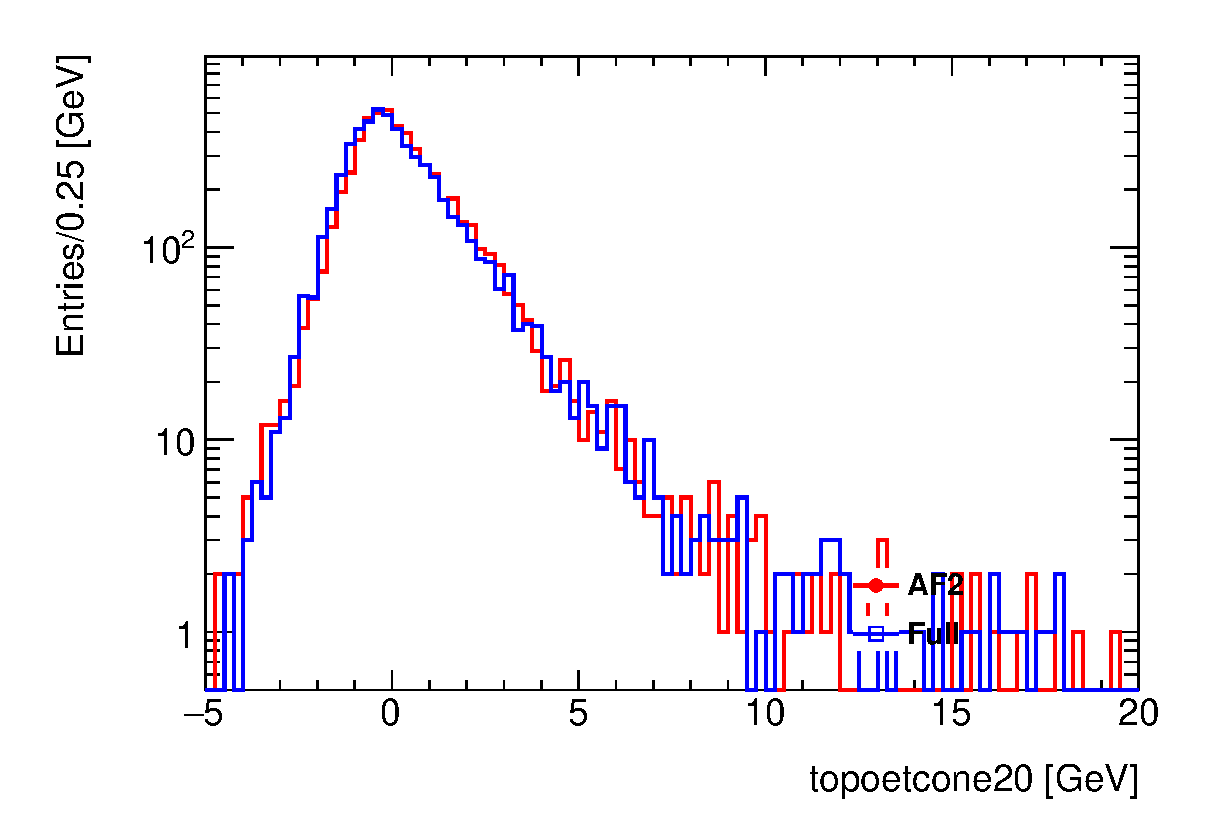
\includegraphics[width=0.5\textwidth]{app/electron_topoetcone20_log}
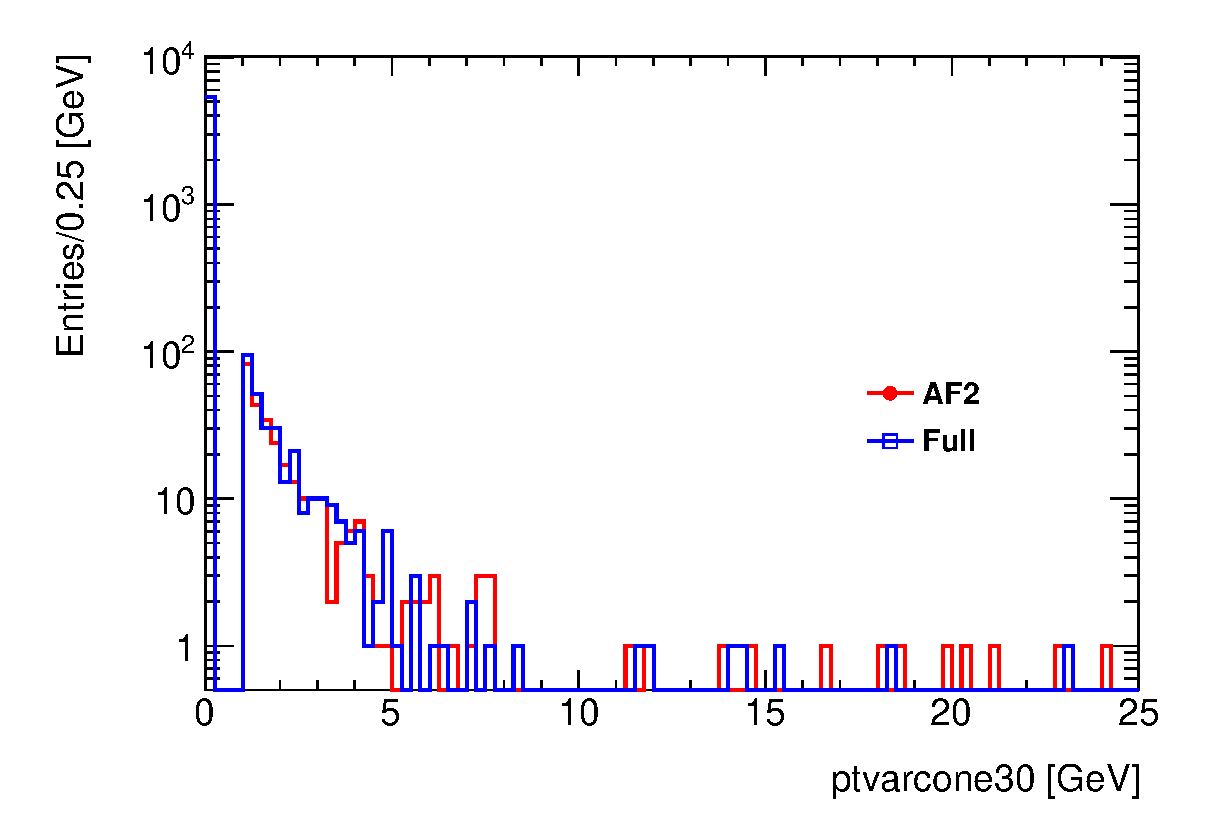
\includegraphics[width=0.5\textwidth]{app/electron_ptvarcone30} 
\caption{Electron isolation variables.}
\label{fig_el_isovar}
\end{figure}

\begin{figure}
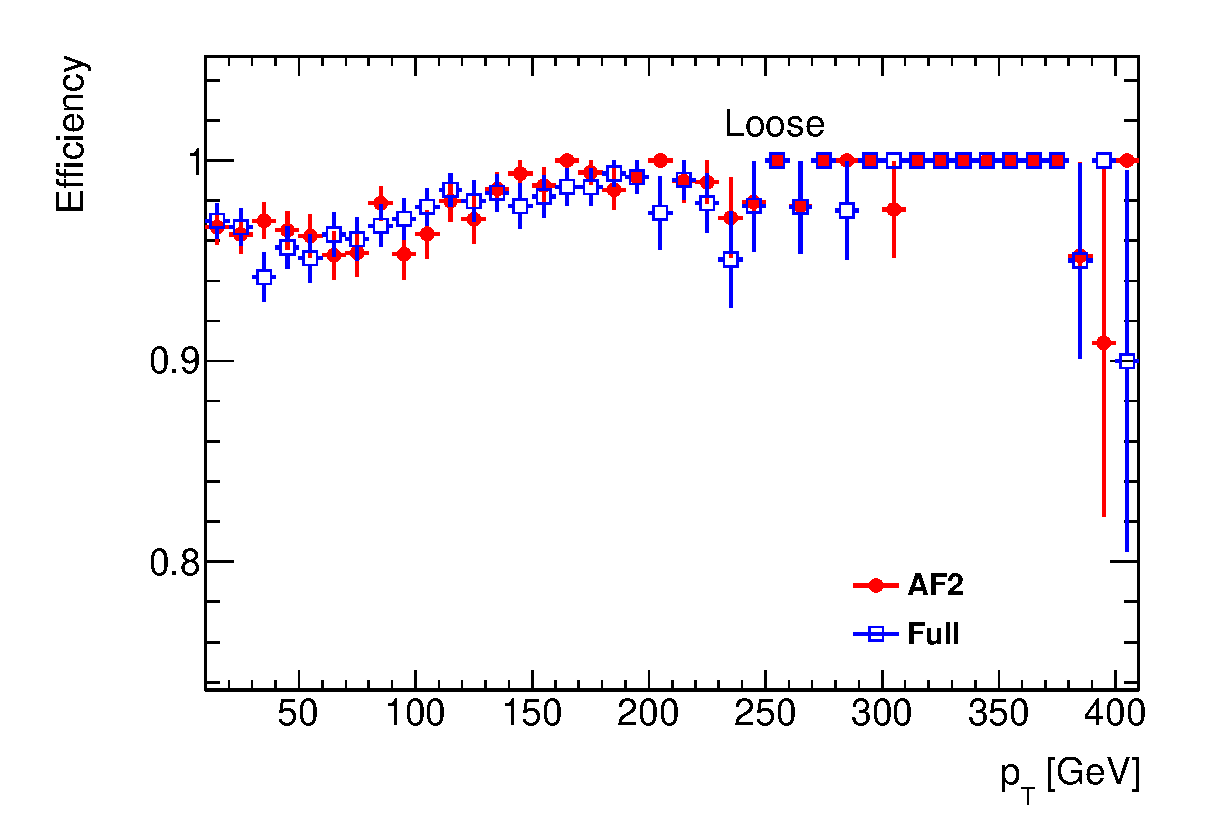
\includegraphics[width=0.5\textwidth]{app/electron_Loose}
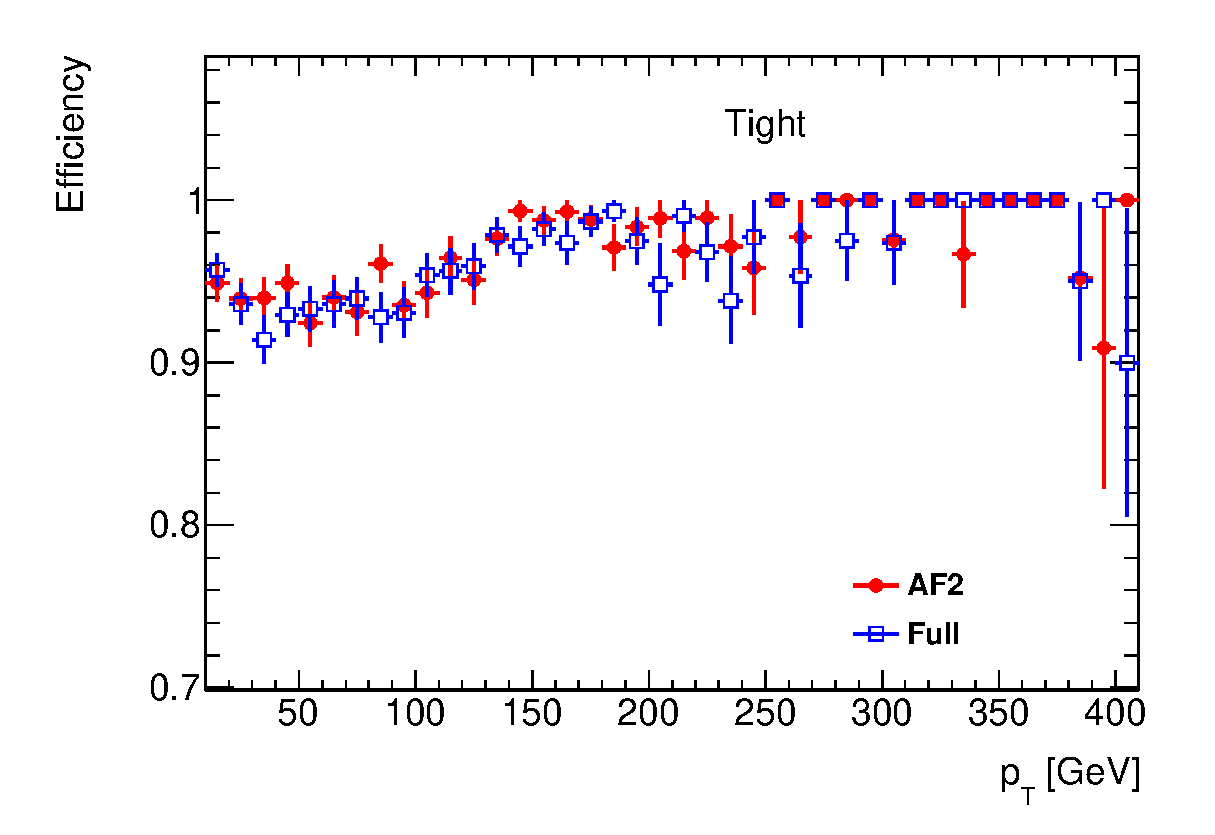
\includegraphics[width=0.5\textwidth]{app/electron_Tight}
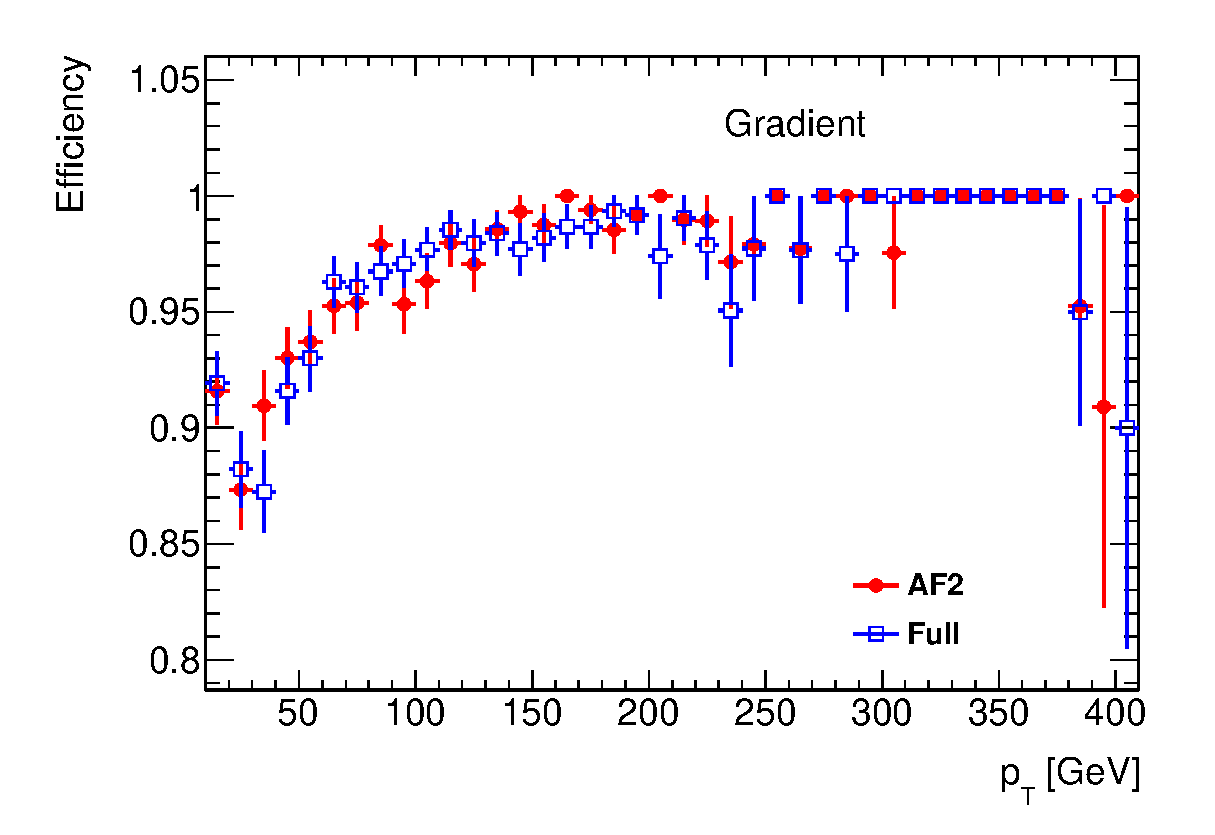
\includegraphics[width=0.5\textwidth]{app/electron_Gradient}
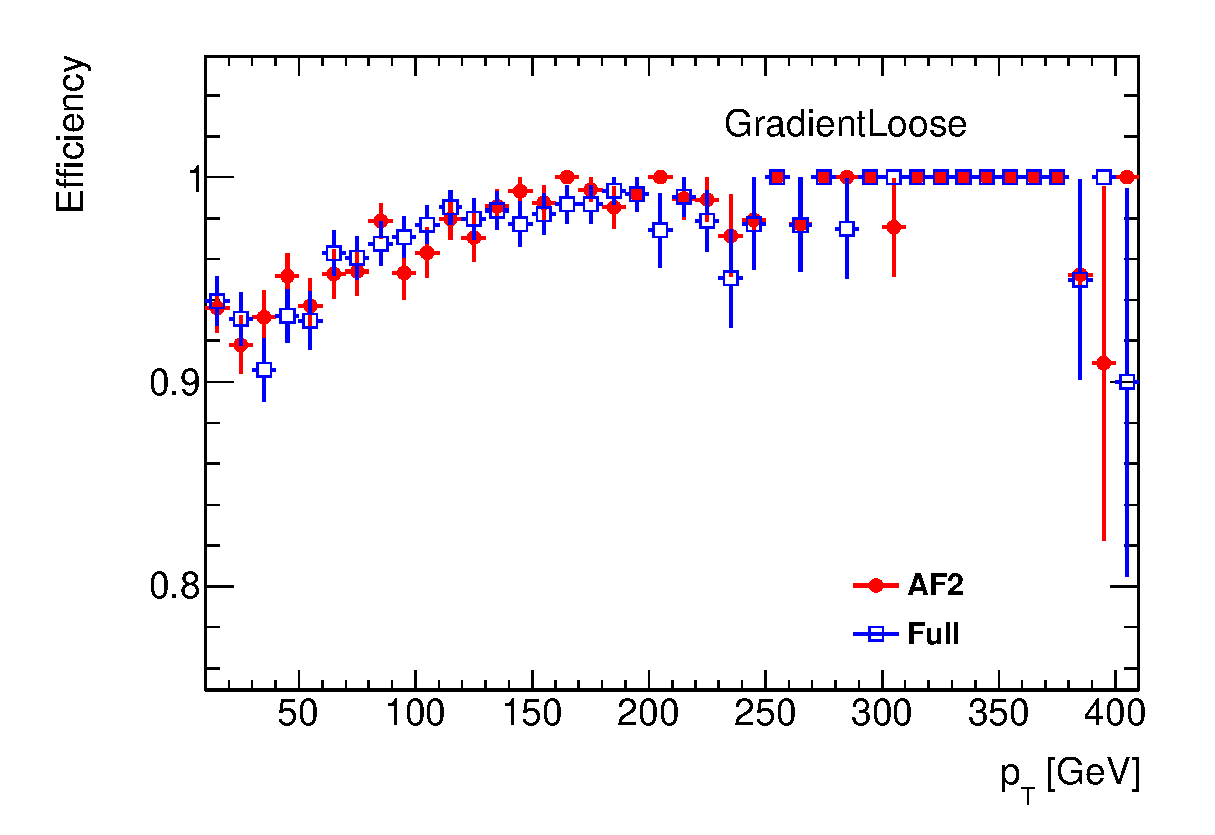
\includegraphics[width=0.5\textwidth]{app/electron_GradientLoose}
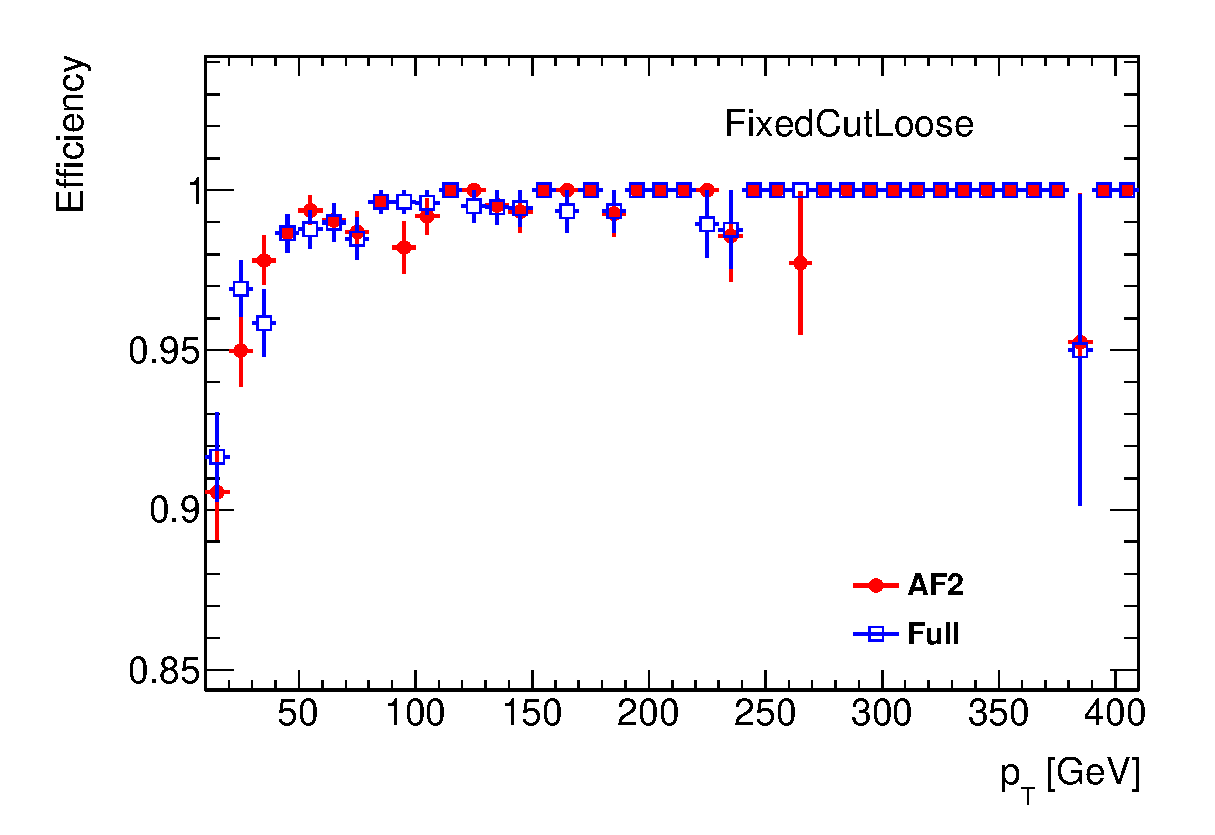
\includegraphics[width=0.5\textwidth]{app/electron_FixedCutLoose}
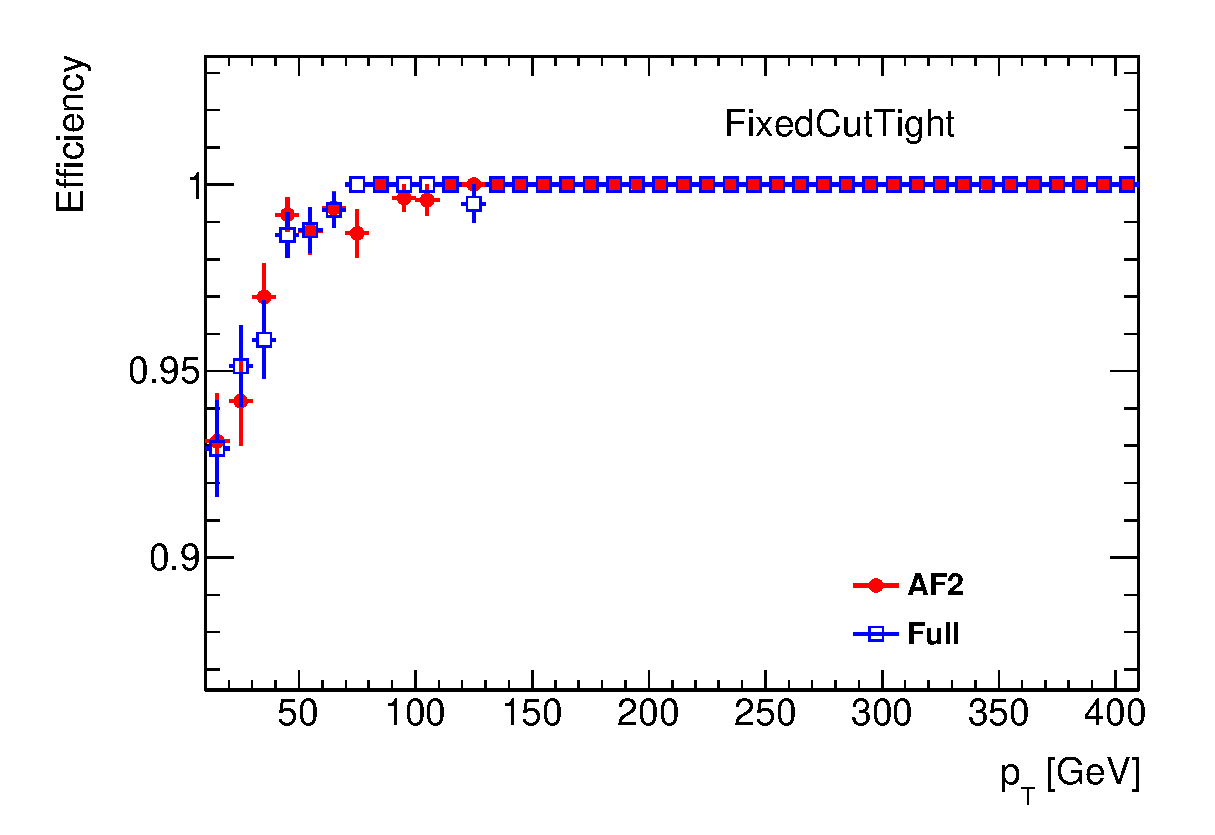
\includegraphics[width=0.5\textwidth]{app/electron_FixedCutTight}
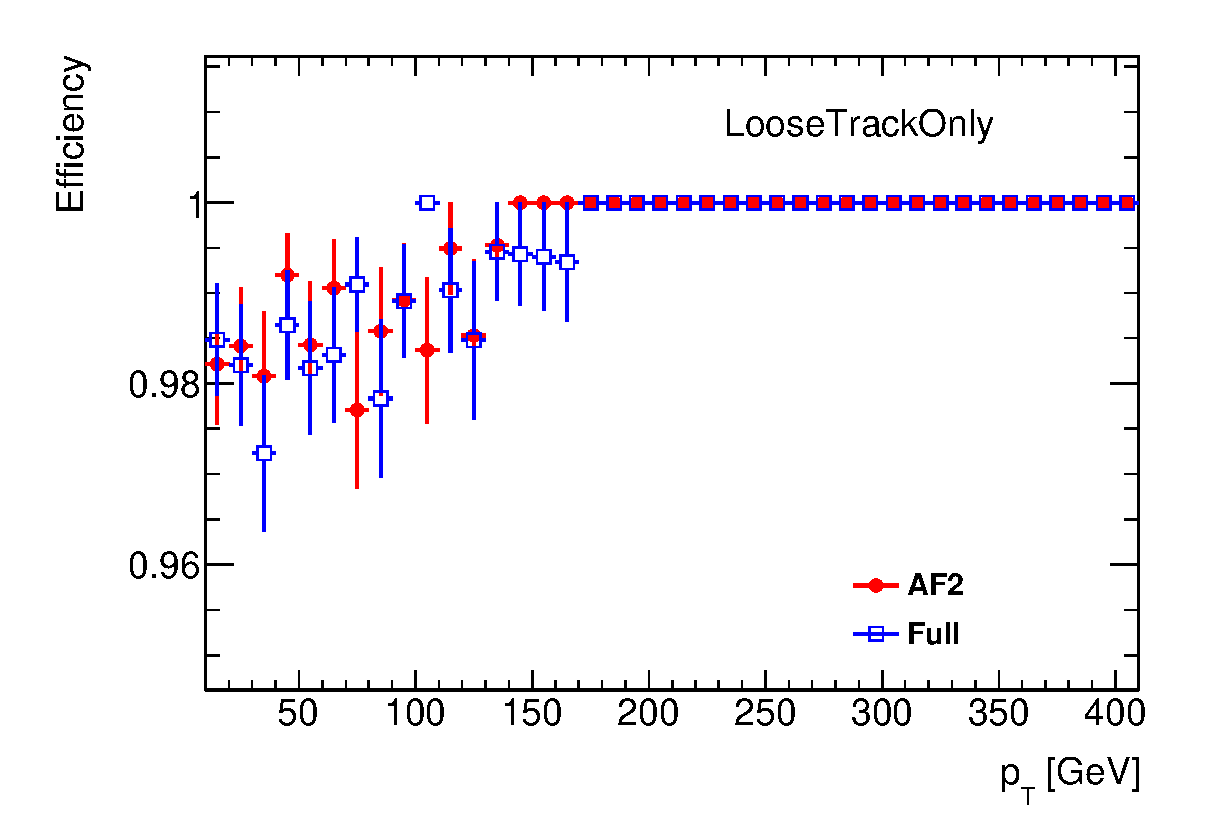
\includegraphics[width=0.5\textwidth]{app/electron_LooseTrackOnly}
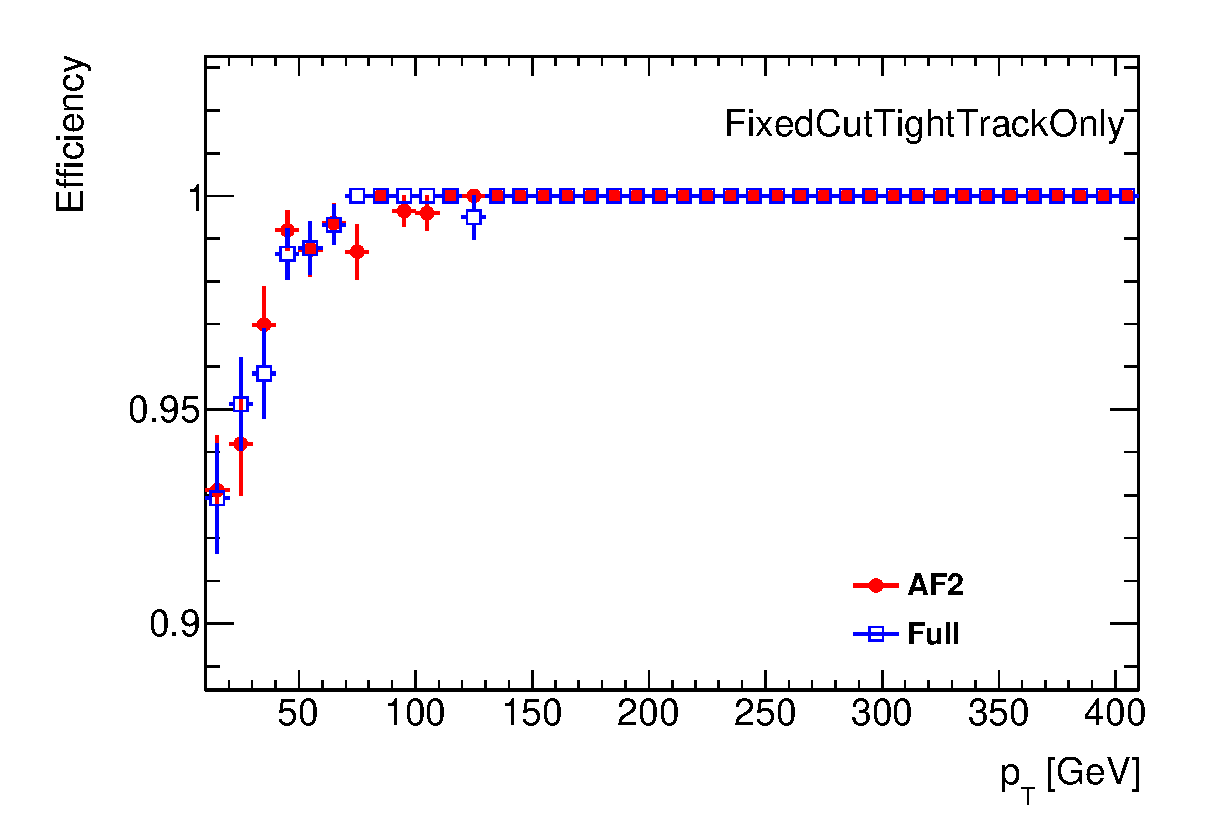
\includegraphics[width=0.5\textwidth]{app/electron_FixedCutTightTrackOnly}
\caption{Electron isolation efficiency comparison.}
\label{fig_el_isoeff}
\end{figure}


\subsection{Muon isolation}
The muon isolation variables are shown in Fig.~\ref{fig_muon_isovar}.
The efficiency comparison for seven muon isolation working points is shown in Fig.~\ref{fig_muon_isoeff}.

\begin{figure}
\includegraphics[width=0.5\textwidth]{app/muon_topoetcone20}
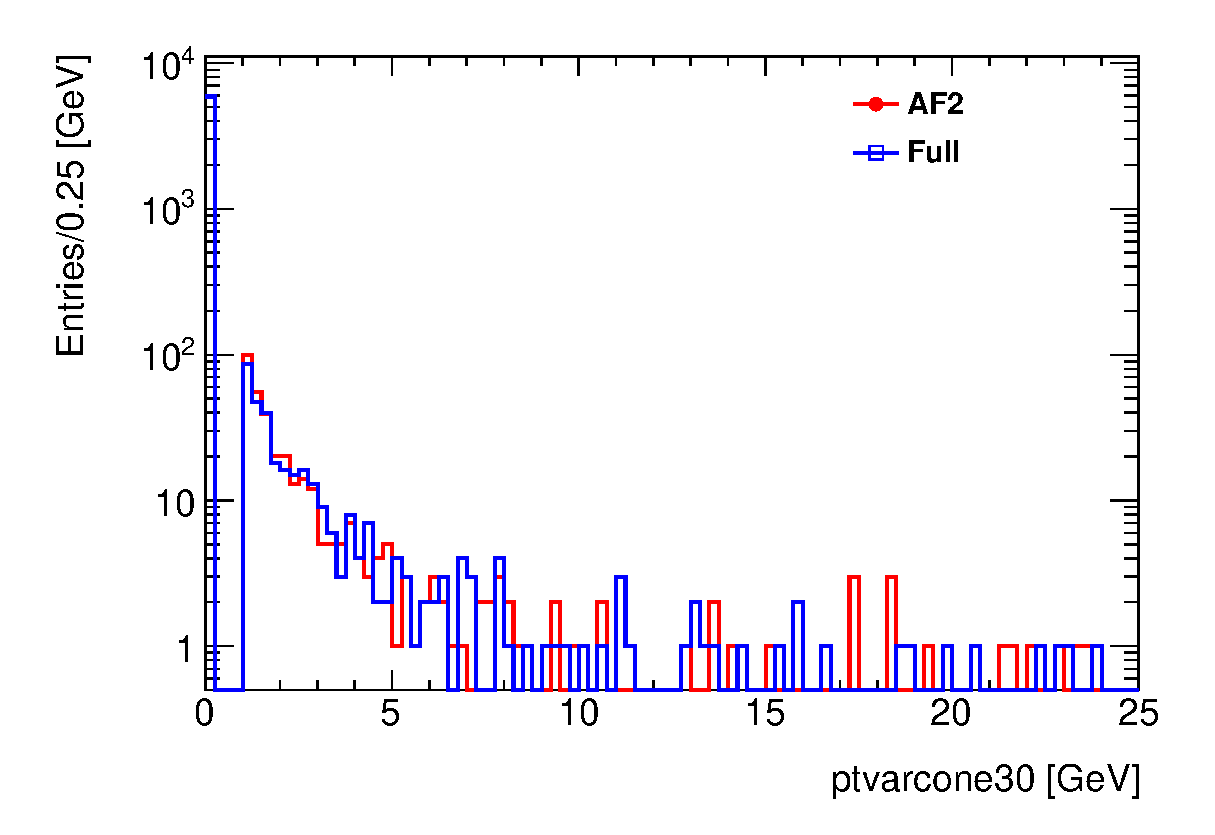
\includegraphics[width=0.5\textwidth]{app/muon_ptvarcone30}
\caption{Muon isolation variables.}
\label{fig_muon_isovar}
\end{figure}

\begin{figure}
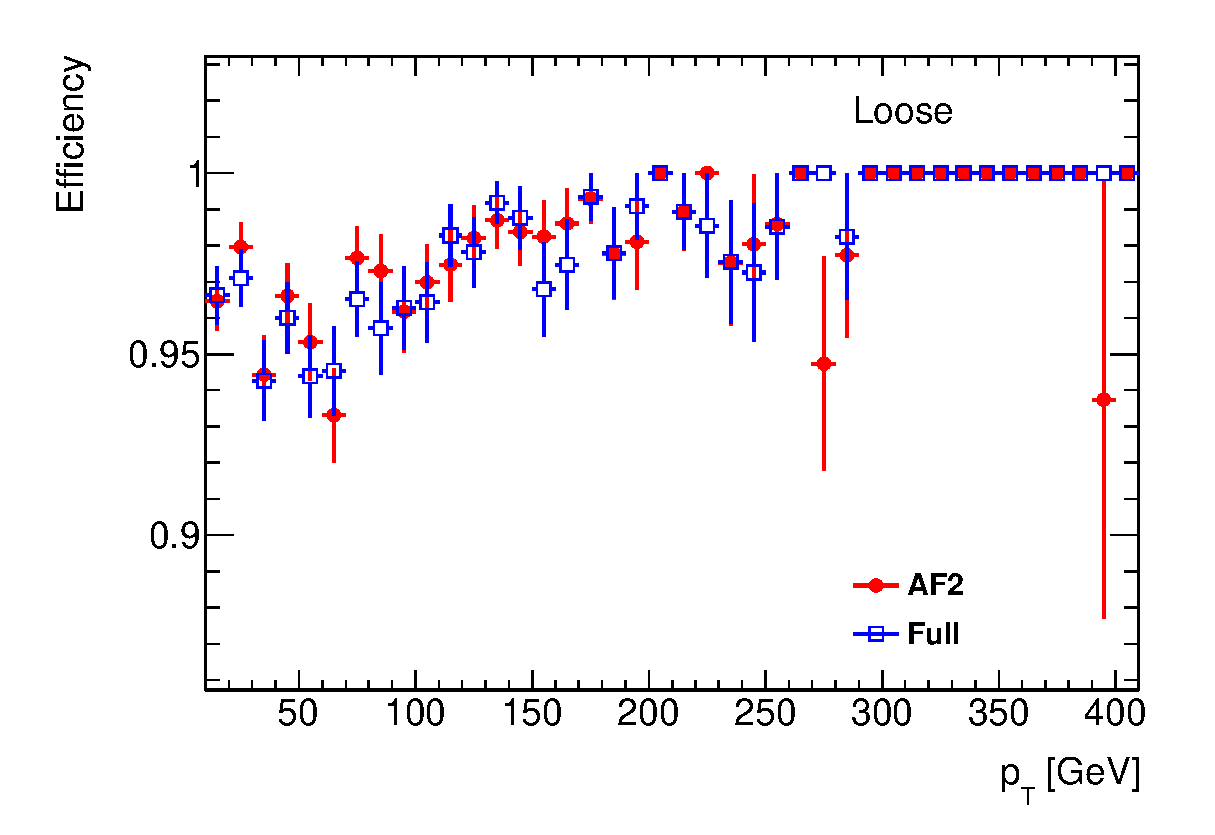
\includegraphics[width=0.5\textwidth]{app/muon_Loose}
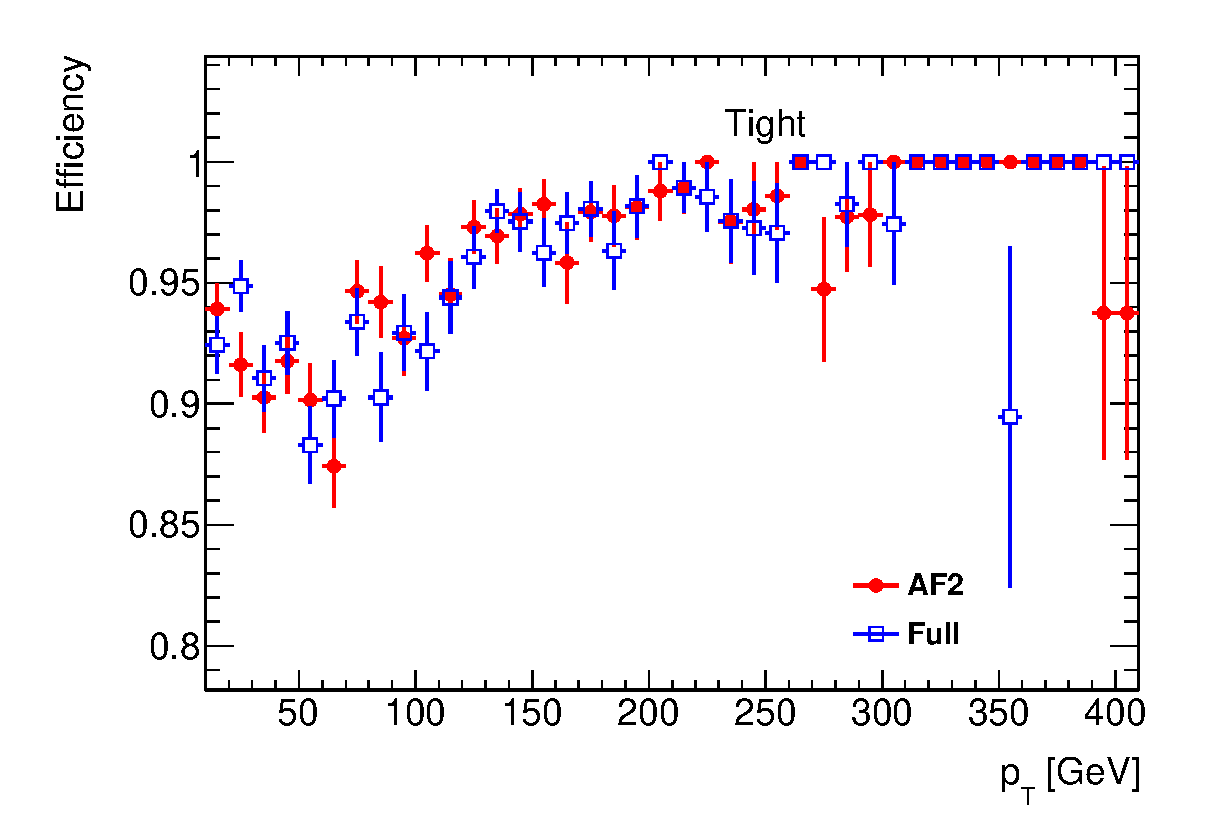
\includegraphics[width=0.5\textwidth]{app/muon_Tight}
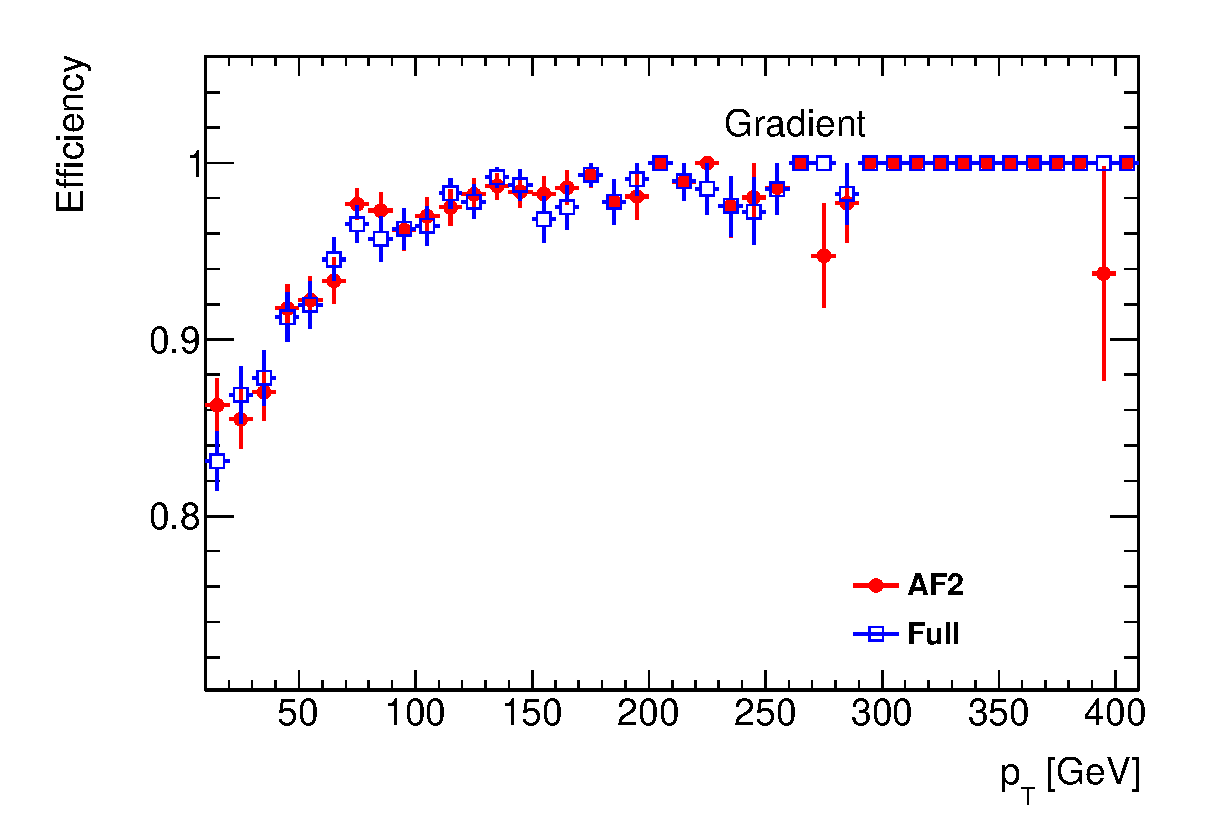
\includegraphics[width=0.5\textwidth]{app/muon_Gradient}
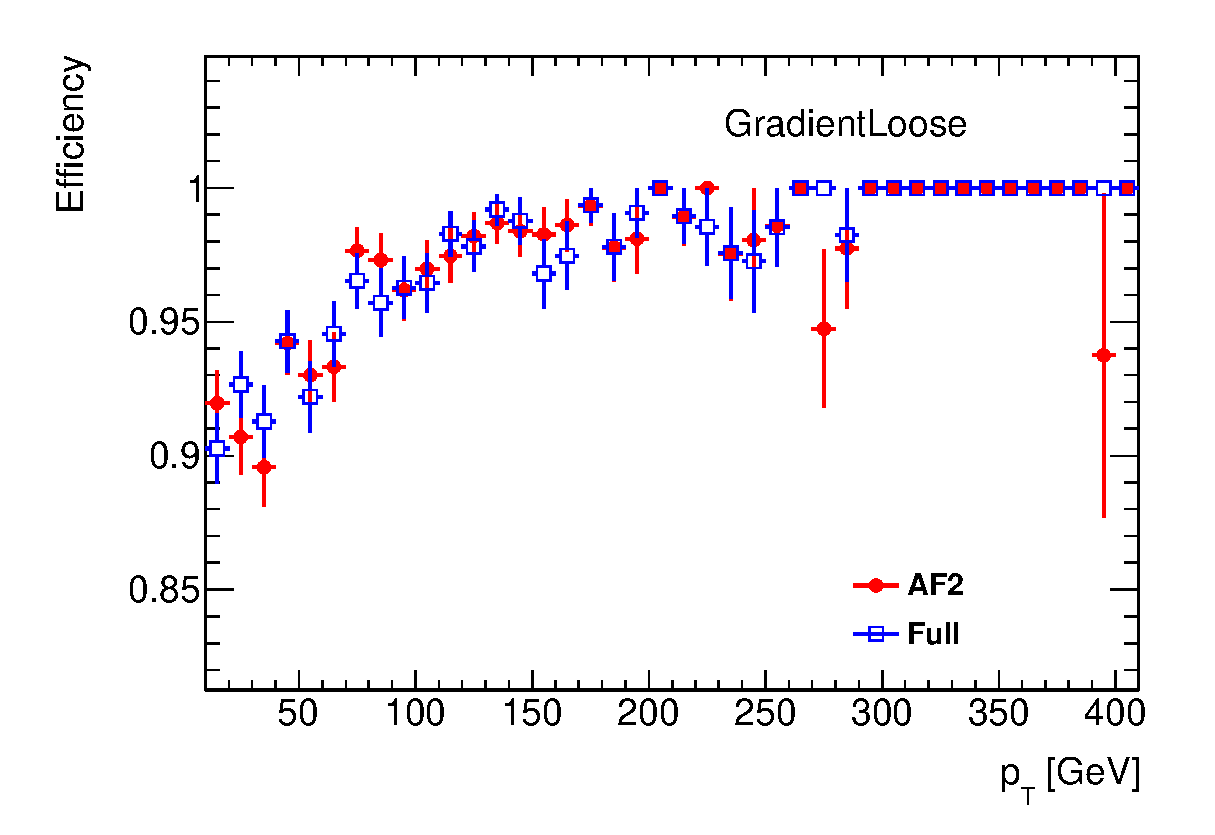
\includegraphics[width=0.5\textwidth]{app/muon_GradientLoose}
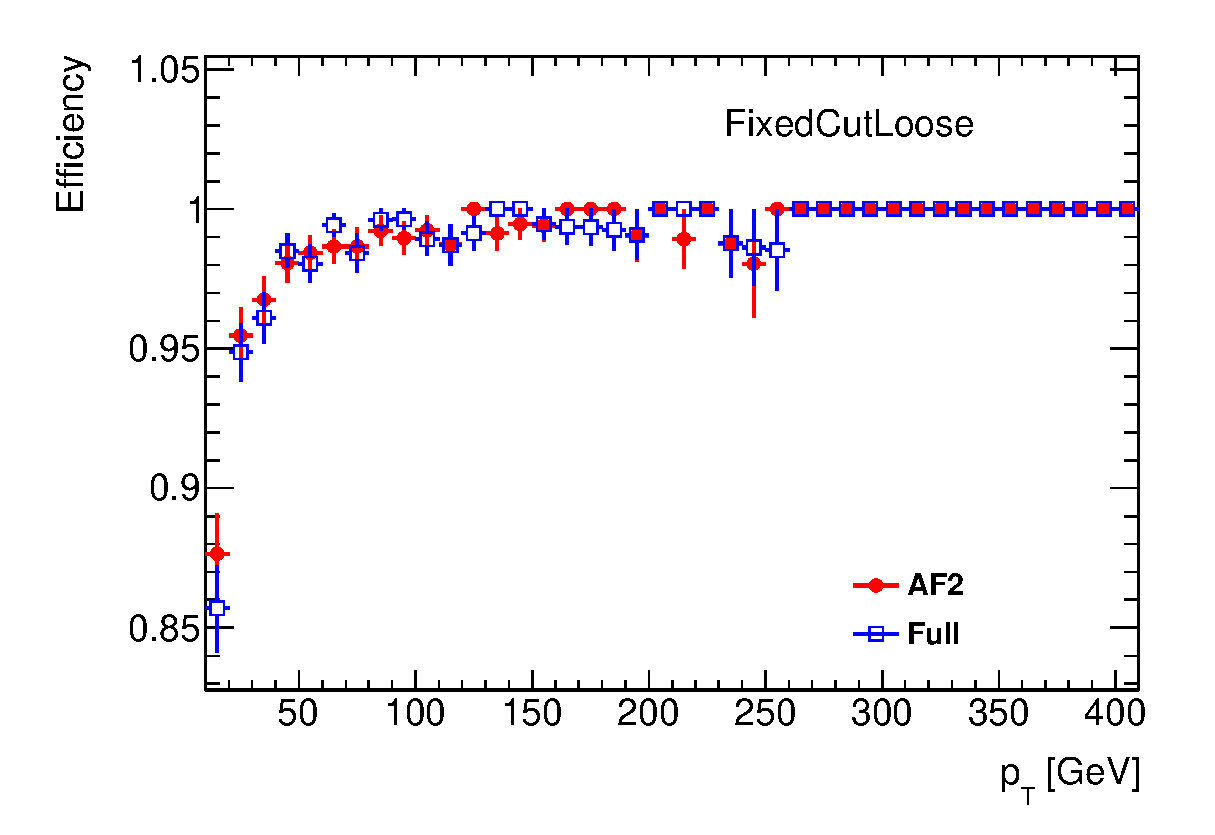
\includegraphics[width=0.5\textwidth]{app/muon_FixedCutLoose}
\includegraphics[width=0.5\textwidth]{app/muon_LooseTrackOnly}
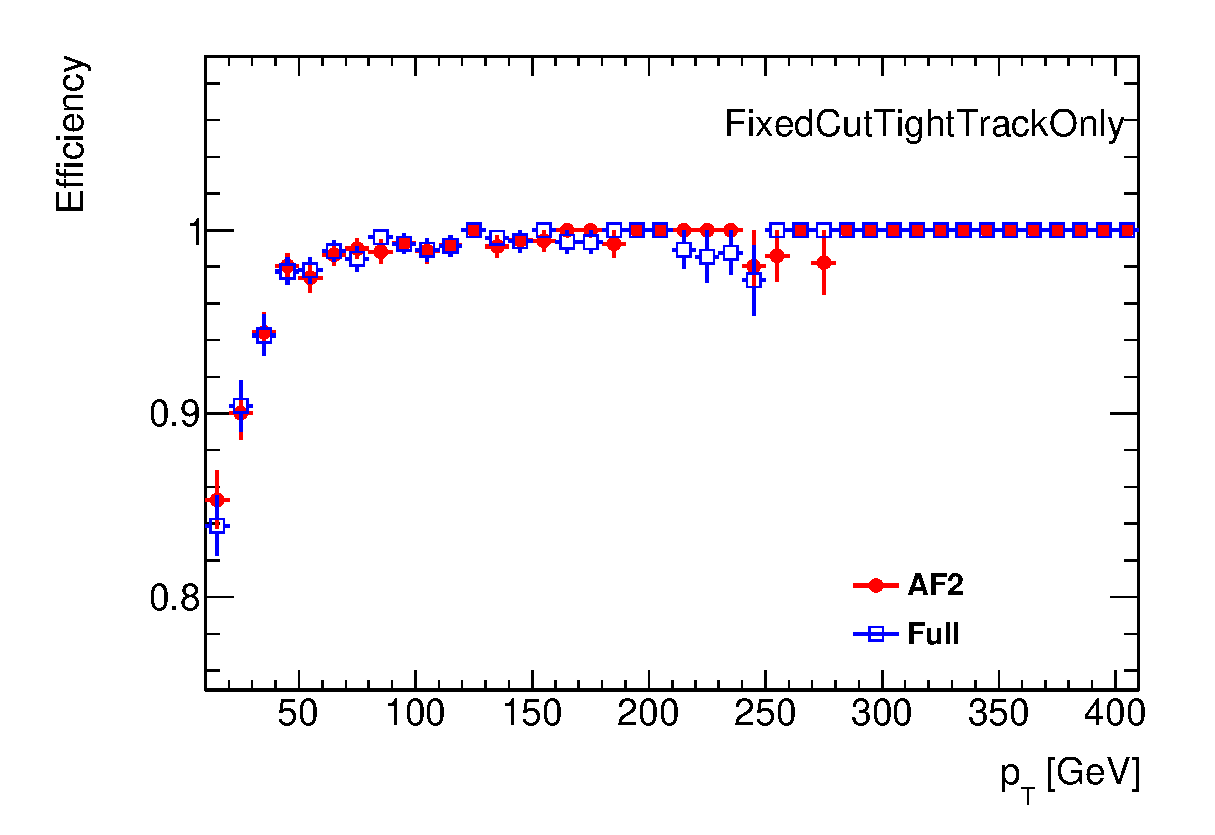
\includegraphics[width=0.5\textwidth]{app/muon_FixedCutTightTrackOnly}
\caption{Muon isolation efficiency comparison.}
\label{fig_muon_isoeff}
\end{figure}


